\chapter{[En curso] Introducción}
\label{chapter:introduccion}

\chapquote{Si he logrado ver más lejos ha sido porque he subido a hombros de gigantes.}{Isaac Newton}

\todo[inline]{Plantear dónde se habla de la introduccion a la salud mental y sus enfermedades}
\todo[inline]{Temas puramente sociales en el contexto?}
\todo[inline]{Estadísticas a tope en la justificación?}
\todo[inline]{Quizás las enfermedades se caracterizen ya en el marco teorico, pero hay que ver (dominio del problema)}

\section{[WIP] Contexto}
    Según la \gls{oms}, se puede definir la salud mental como ``un estado de bienestar mental que permite a las personas hacer frente a los momentos de estrés de la vida, desarrollar todas sus habilidades, poder aprender y trabajar adecuadamente y contribuir a la mejora de su comunidad`` \cite{oms_salud_2022}. Por tanto, es parte integral de la salud y el bienestar de una persona; tal y como reflejada en la definición de salud de la propia \gls{oms}: “La salud es un estado de completo bienestar físico, mental y social, y no solamente la ausencia de afecciones o enfermedades” \cite{feafes_galicia_que_nodate}.

    Asimismo, el bienestar emocional se puede concebir como ``el conjunto de sensaciones positivas derivadas de un funcionamiento mental que nos capacita para hacer frente o adaptarnos a las situaciones y demandas ambientales`` \cite{clinic_barcelona_que_nodate}. \footnote{Como el lector quizá se haya dado cuenta, la Salud Mental y el Bienestar Emocional son conceptos relativamente similares, por lo que se usarán indistintamente a lo largo de esta sección si el contexto lo permite.}

    Las estadísticas sobre la salud mental arrojan una preocupante tendencia de cara al futuro, tanto a nivel nacional como internacional. Según el informe ``La situación de la Salud Mental en España 2023`` \cite{comunicacion_cuatro_2023}, realizado con la colaboración de más de 2.000 personas, el 39,3\% de las personas valoraban de forma negativa su salud mental actual. Asimismo, el 42,1\% han sufrido una depresión a lo largo de su vida, mientras que un 36,9\%, ansiedad prolongada en el tiempo. 
    
    
    Por otra parte, se estima a nivel mundial una de cada cuatro personas tendrán un trastorno mental a lo largo de su vida, mientras que en España, casi la mitad de los y las jóvenes de entre 15 y 29 años (48,9\%) considera que ha tenido algún problema de salud mental.


    ----

    Por otra parte, existen numerosos trastornos o enfermedades mentales que afectan a la salud mental. En la propia definición de salud mental se menciona el estrés, el cual se puede entiende como ``un estado de preocupación o tensión mental generado por una situación difícil`` \cite{oms_estres_2023}. La presencia de estrés puede provocar, entre otros, dolor de cabeza, dificultades para dormir, alternaciones del apetito u otros problemas de salud mental, como ansiedad \cite{oms_estres_2023}. Se estima que nueve de cada diez personas han sentido estrés en el último año y un 40\% de la población lo sufre de forma continua \cite{nogera_mas_estres_2024}.

    Otro problema de salud mental muy conocido es la depresión, la cual está muy relacionada con el estrés, la cual se puede describir como un estado de intensa tristeza, melancolía o desesperación, avanzada hasta perturbar el funcionamiento social o las actividades diarias de una persona \cite{van_neerven_rarrxr_2008}. 



    

\section{[WIP] Justificación}
    
    Desafortunadamente, no se puede entender la salud mental sin la gran estigmatización que ha sufrido y sin los prejuicios hacia las enfermedades y los pacientes que las sufren \cite{delgado_rompiendo_2021} \cite{andres_tallarda_combatir_2020}. Según la Fundación de Salud Mental de Inglaterra, nueve de cada diez personas que sufren algún problema de Salud Mental se han visto afectadas negativamente por el estigma o la discriminación \cite{mental_health_foundation_stigma_nodate}.

    Si bien en los últimos años la salud mental ha ganado visibilidad y atención, gracias a iniciativas como la creación del Observatorio Estatal de Salud Mental, Derechos e Igualdad \cite{comunicacion_nace_2022} o la concienciación por parte de individuos particulares; continúa siendo un problema relativamente oculto que afecta profundamente a nuestra sociedad y que no se está resolviendo correctamente. 
    
    Según estadísticas de la Confederación Salud Mental España \cite{confederacion_salud_mental_espana_salud_nodate} \cite{aguilar_laura_2022}, en España más de la mitad de las de las personas con trastorno mental que necesitan tratamiento no lo reciben, y un porcentaje significativo no recibe el adecuado. Más de la mitad (58,5\%) de las personas diagnosticadas con un problema de salud mental ha sentido rechazo social por ello en algún momento de su vida, mientras que un 11\%, no ha comunicado a nadie su problema.
    
    
    En el caso de que el paciente busque ayuda, no se vislumbra un entorno muy halagüeño, ya que en nuestro país solo se disponen en la Sanidad Pública de seis psicólogos por cada 100.000 habitantes \cite{antolin_listas_2023}; muy por debajo de países de nuestro entorno como Alemania (41) o Francia (15), entre otros. Asimismo, las listas de espera dentro de la sanidad pública, tal y como se pueden ver en la Figura \ref{fig:intro:dias_espera}, provocan que la salud mental se perciba como poco menos que un lujo. Para el 57,3\% de la población \cite{comunicacion_cuatro_2023}, acudir a un profesional de la salud mental privado es económicamente inaccesible.
    
    \begin{figure}[h]
        \centering
        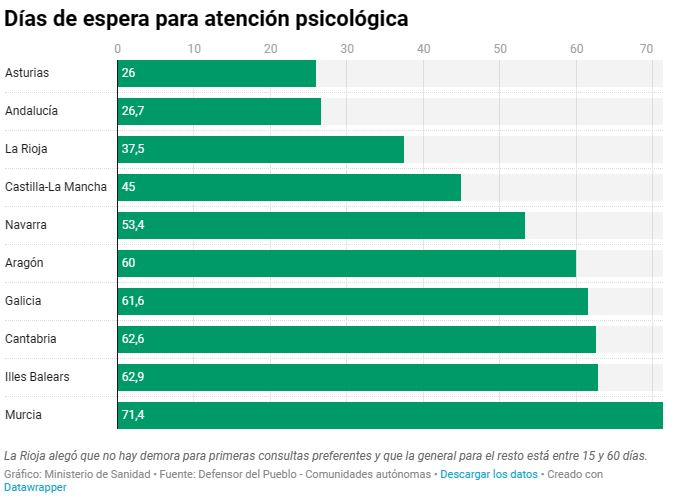
\includegraphics[width=0.75\linewidth]{figures/dias espera.JPG}
        \caption[Días de espera para atención psicológica según Comunidades Autónomas]{Días de espera para atención psicológica según Comunidades Autónomas \cite{asuar_gallego_recurrir_2021}}
        \label{fig:intro:dias_espera}
    \end{figure}

    Por otra parte, las enfermedades mentales afectan a todo tipo de personas. Algunas personas que la sociedad percibe como exitosas han sufrido problemas de salud mental, desde ``pequeños`` brotes como Alejandro Sanz \cite{lopez_chicon_que_2023} \cite{riano_alejandro_2023}, hasta casos de suicidio, como el del cantante Chester Bennington, el cual experimentó depresión durante largas fases de su vida \cite{el_universal_nada_2020} \cite{gambin_historia_2022}.

    Quizás una de los efectos más visibles de los problemas de salud mental sea el suicidio. Si se dirige la mirada hacia las redes sociales, se pueden encontrarse duros testimonios de personas a los que el suicidio arrebató de sus vidas a un ser querido, los cuales sencillamente transcienden de las estadísticas; tal y como se puede ver en la Figura \ref{fig:intro_testimonio_madre} .
    
    \begin{figure}[h]
        \begin{subfigure}[b]{0.49\textwidth}
            
\includegraphics[width=1\linewidth]{figures/testimonio_madre_1.jpg}
        \end{subfigure}
        \hfill
        \begin{subfigure}[b]{0.49\textwidth}
            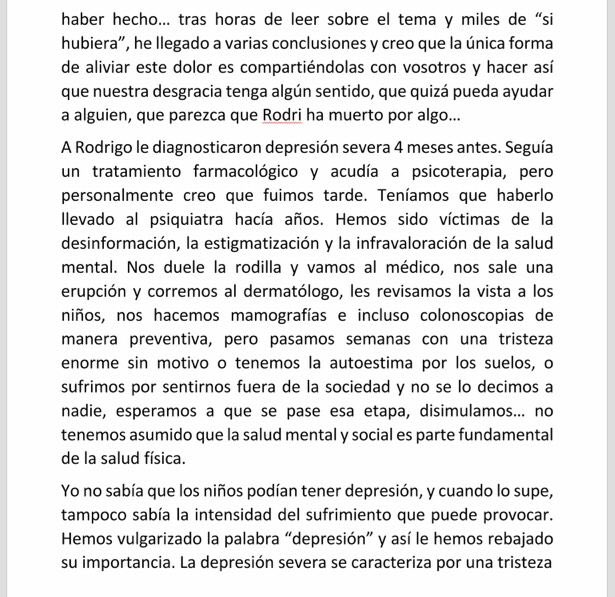
\includegraphics[width=1\linewidth]{figures/testimonio_madre_2.jpg}
        \end{subfigure}
        \caption[Extracto del testimonio de una madre tras el suicidio de su hijo]{Extracto del testimonio de una madre tras el suicidio de su hijo \cite{irene_pujol_i_athenea_hace_2021}}
        \label{fig:intro_testimonio_madre}
    \end{figure}

    No obstante, si se acude a las estadísticas, en España, durante 2022 se suicidaron 4.227 personas. En otras palabras, once vidas perdidas cada día. Una estadística absolutamente demoledora que desde 2018, no para de aumentar (ver Figura \ref{fig:intro:muertes_suicidio}).
    
    \begin{figure}[h]
        \centering
        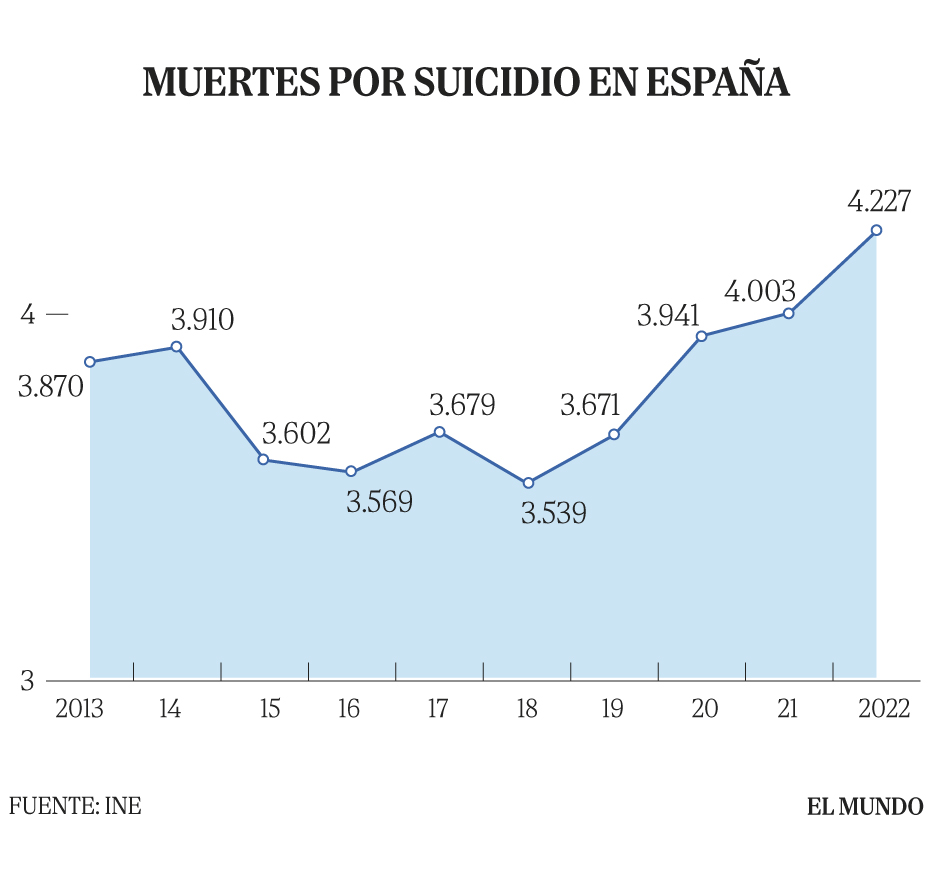
\includegraphics[width=0.66\linewidth]{figures/muertes_suicidio.jpg}
        \caption[Muertes por suicidio en España desde 2013 hasta 2022]{Muertes por suicidio en España desde 2013 hasta 2022 \cite{saiz_4227_2023}}
        \label{fig:intro:muertes_suicidio}
    \end{figure}

    El suicidio se mantiene como primera causa no natural de muerte en nuestro país desde 2008, por encima de otras quizá más presentes en el imaginario colectivo, como los accidentes de tráfico o los ahogamientos (ver Figura \ref{fig:intro:causas_no_naturales}).  En el mundo, cerca de 800.000 personas se suicidan \textbf{cada año}, siendo la segunda causa de muerte entre los jóvenes de 16 a 29 años. \cite{confederacion_salud_mental_espana_salud_nodate}
    
    \begin{figure}[h]
        \centering
        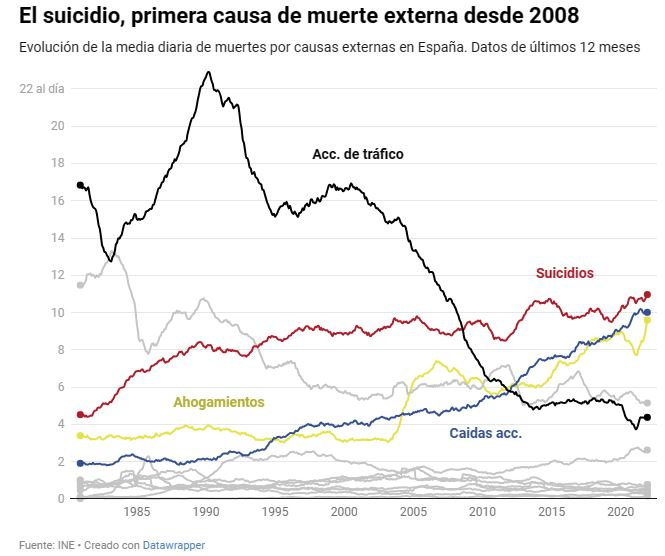
\includegraphics[width=0.85\linewidth]{figures/causas no naturales.jpg}
        \caption[Evolución de la media diaria de las muertes por causas no naturales en España, desde 1980 a 2021]{Evolución de la media diaria de las muertes por causas no naturales en España, desde 1980 a 2021 \cite{sanchez_once_2023}}
        \label{fig:intro:causas_no_naturales}
    \end{figure}

     No obstante, esta funesta métrica solo muestra a las personas que desgraciadamente decidieron acabar con su vida, sin mostrar los casos de personas que sufren en vida. Sin ir más lejos, según el catedrático en Psiquiatría Jose Luis Ayuso Mateos ``por cada persona que fallece, hay 25 que lo han intentado``  \cite{sanchez_once_2023}.  Por otra parte el 14,5\% de la población ha tenido ideas suicidas o lo ha intentado \cite{comunicacion_cuatro_2023}.

    -----

    Sus consecuencias y estadísticas, como veremos a continuación, son demoledoras; y que en muchas ocasiones continua siendo un tema tabú. Transciende mucho más allá de ``simples`` pensamientos de angustia o tristeza, siendo una cuestión que, como sociedad, no estamos siendo capaces de solucionar.
    
    
   

    


\section{Motivación}

    Si se ahonda en el bienestar emocional dentro de la comunidad universitaria, se puede tomar como punto de partida el informe realizado por el Ministerio de Universidades en colaboración con el Ministerio de Sanidad: ``La salud mental en el estudiantado de las universidades españoles`` \cite{galache_gobierno_2023} \cite{ministerio_de_universidades_salud_2023}, de recomendada lectura. El nombrado estudio fue realizado en dos fases en su parte cuantitativa, correspondiendo las fases respectivas al final de los cuatrimestres 1 y 2 del curso 2022-23. 
    
    En él, se detalla que en las últimas dos semanas, aproximadamente la mitad de los estudiantes presentaron síntomas depresivos, mientras que la ideación suicida estaba presente en aproximadamente uno de cada cinco, como se puede ver en la Figura \ref{fig:intro:sintomas_depresivos_suicida}. 
    
    \begin{figure}[h]
        \centering
        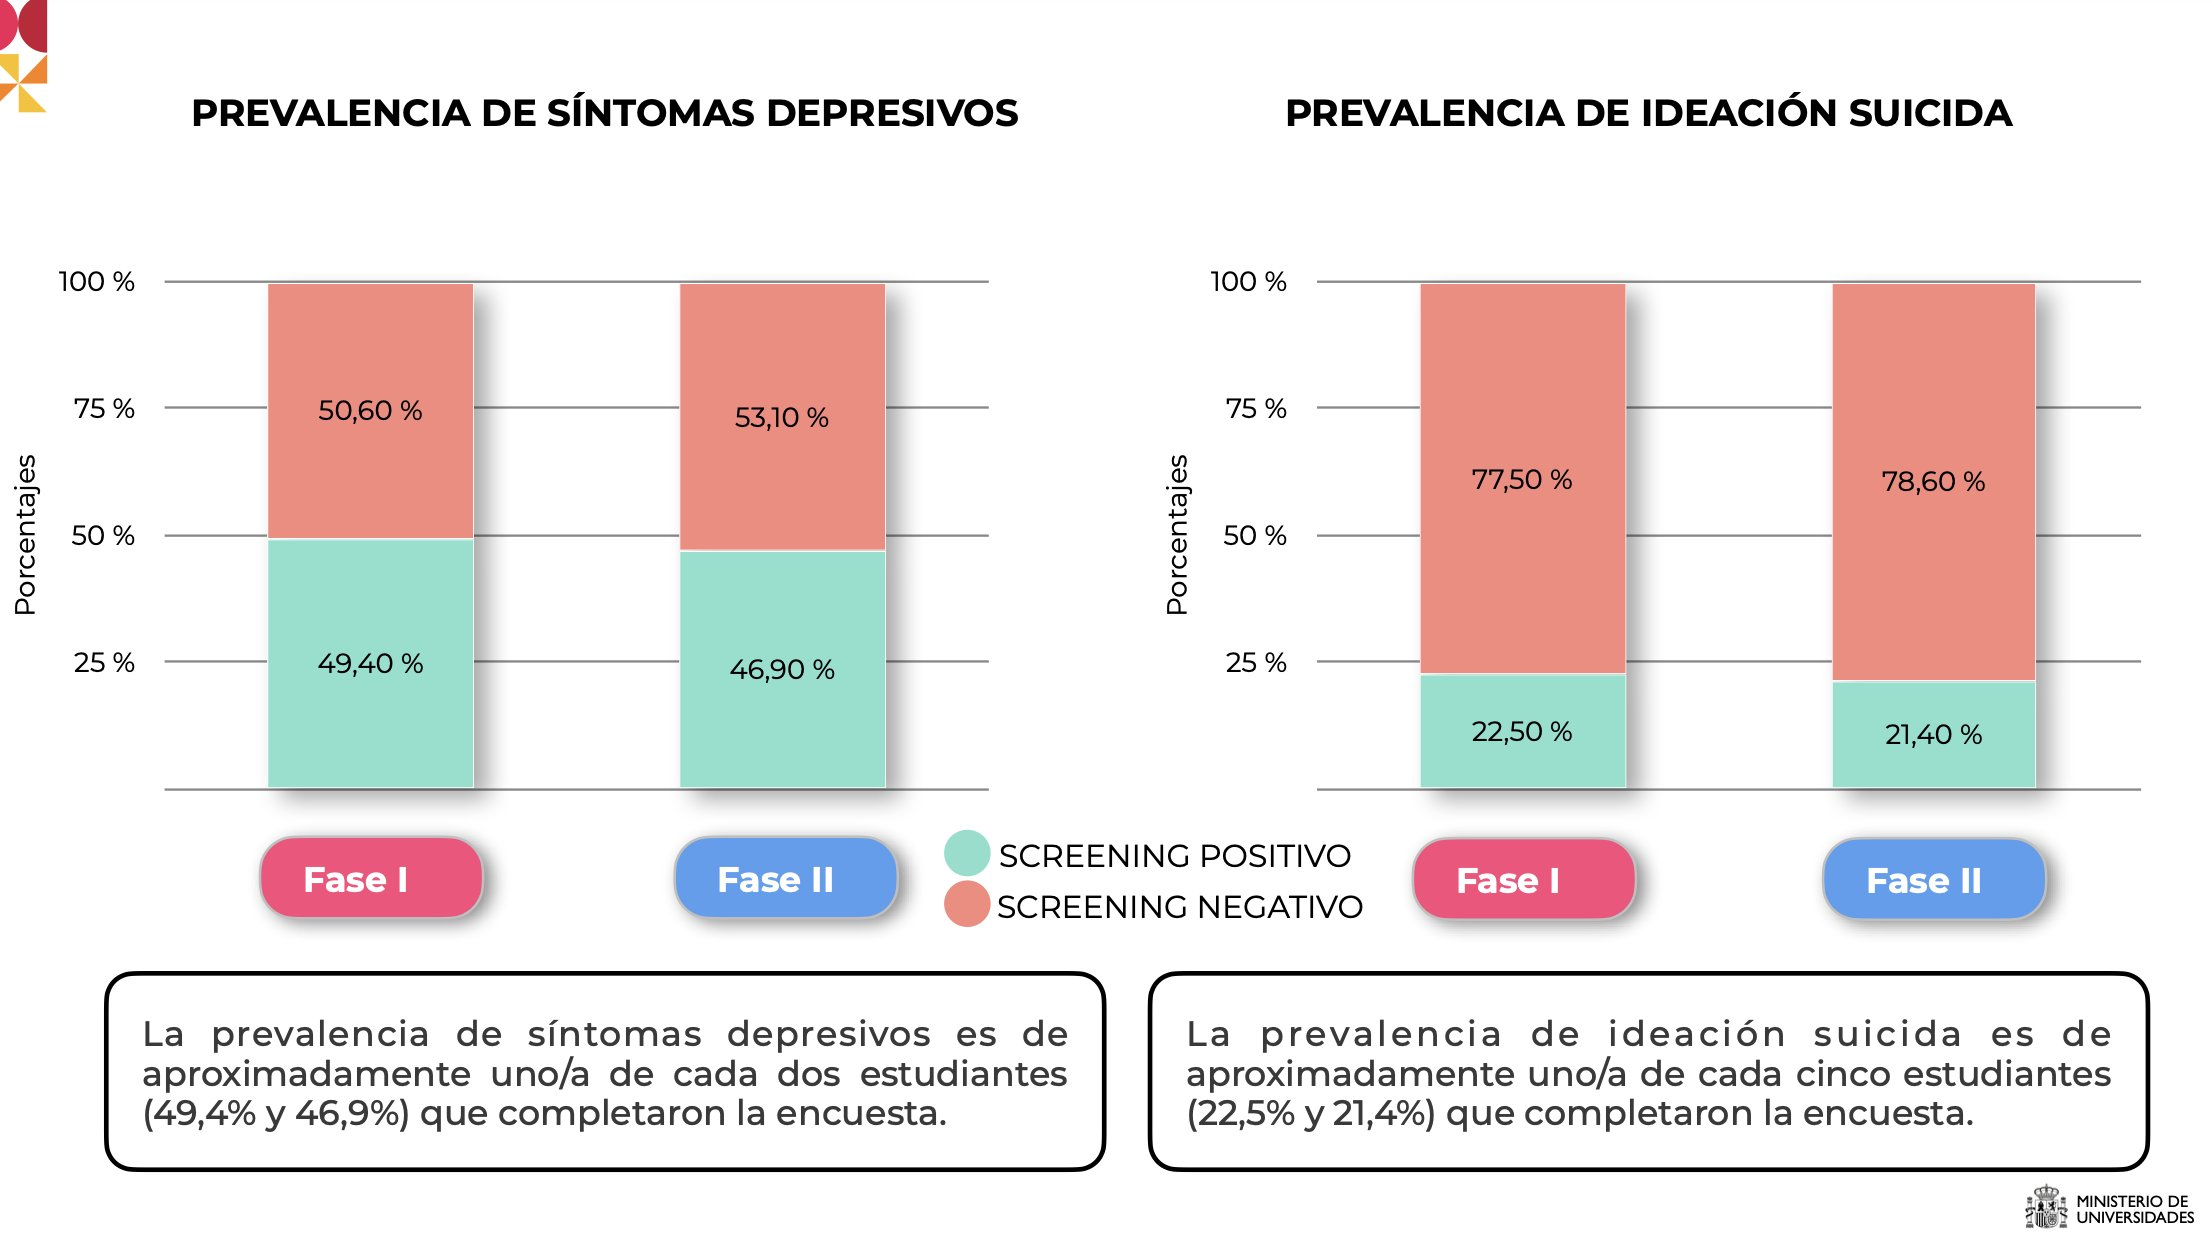
\includegraphics[width=0.75\linewidth]{figures/Sintomas depresion suicidio.jpg}
        \caption[Prevalencia de síntomas depresivos e ideación suicida]{Prevalencia de síntomas depresivos e ideación suicida \cite{ministerio_de_universidades_salud_2023}}
        \label{fig:intro:sintomas_depresivos_suicida}
    \end{figure}
    
    En cuanto a la prevalencia de ansiedad moderada o grave encontramos que una de cada dos personas la han sufrido en las últimas dos semanas, mientras que uno de cada cinco presenta insomnio clínico o grave, como se puede ver en la figura \ref{fig:intro:sintomas_ansiedad_insomnio}. 
    
    \begin{figure}[h]
        \centering
        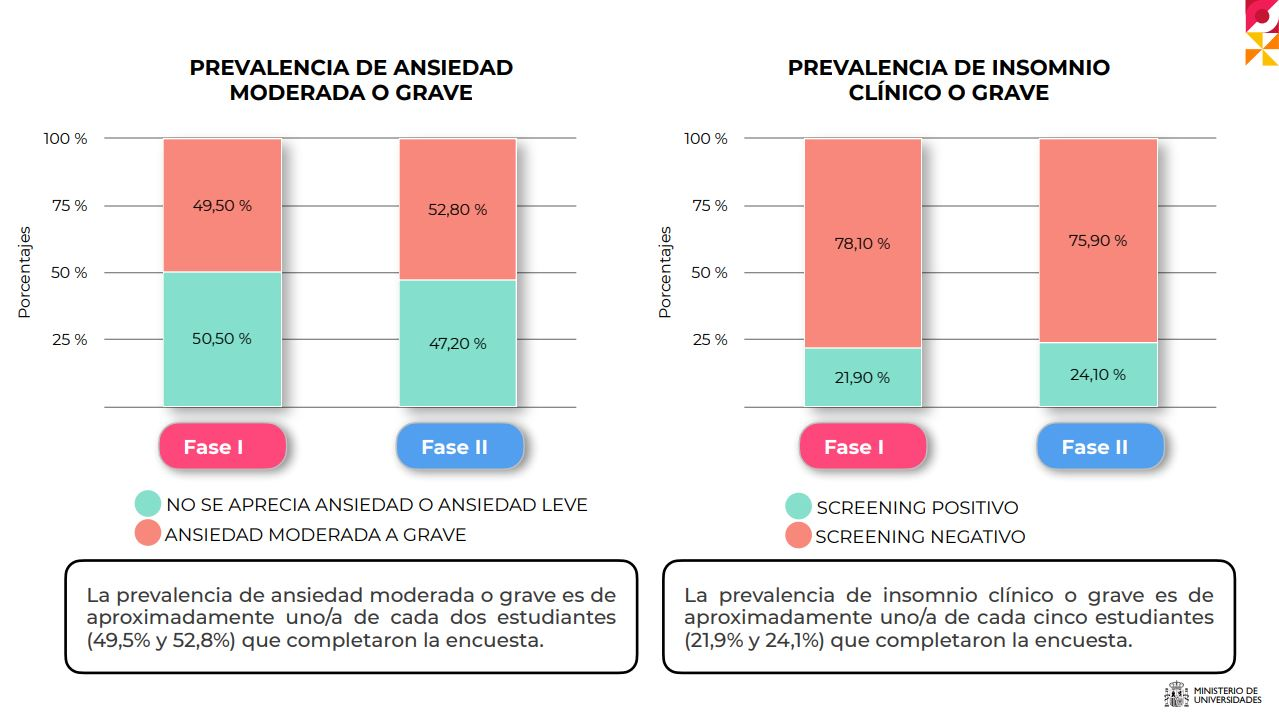
\includegraphics[width=0.75\linewidth]{figures/Sintomas ansiedad insomnio.JPG}
        \caption[Prevalencia de síntomas de ansiedad e insomnio graves]{Prevalencia de síntomas de ansiedad e insomnio graves \cite{ministerio_de_universidades_salud_2023}}
        \label{fig:intro:sintomas_ansiedad_insomnio}
    \end{figure}
    
    La sección cualitativa muestra una vez más los problemas que ``disponen'' los estudiantes para acceder al apoyo psicológico, nombrando barreras como las listas de espera o el número limitado de sesiones, o la soledad en la realización del doctorado.
    
    Estos datos ponen de manifiesto, tanto dentro como fuera de la comunidad universitaria la necesidad crítica de trabajar tanto en la prevención, en el diagnóstico precoz y en la atención a las personas que sufren un trastorno mental que, bien por desconocimiento o por estigma, no reciben el tratamiento que necesitan.
    
    En esta necesidad fehaciente se sitúan numerosas iniciativas, como ``Special Initiative for Mental Health (2019-2023)`` \cite{oms_salud_nodate} de la OMS, o dentro de España, la ``Estrategia de Salud Mental`` o la línea 024 de atención a la conducta suicida \cite{la_moncloa_minones_2023}.

    Otra cuestión es la relación de la Informática con la Salud Mental, tema de actual debate en la comunidad científica. El uso de redes sociales podría afectar a nuestra salud mental \cite{burn-murdoch_smartphones_2023}. Algunos argumentos que ratificarían esa afirmación son un espectacular incremento de los ratios de suicidio en jóvenes desde la popularización de los \textit{smartphones} y redes sociales en Estados Unidos como en Reino Unido, o la multiplicación por 4 de los ratios de depresión en Francia entre las personas de 15 a 24 años en la última década.
    
    Por otra parte, la popularización de los \textit{smartphones} y de los \glspl{wearable} permiten obtener más información sobre el comportamiento de la persona (uso del móvil, ejercicio físico, hábitos de sueño), sus constantes vitales (pulsaciones, niveles de oxígeno en sangre), lo que podría ayudar a la detección precoz de problemas de salud mental.
    
    En definitiva, puede apreciarse que las enfermedades mentales son un problema muy relevante en nuestra sociedad, a la vez que transversal. Ante tales hechos y estadísticas, urge que las personas afectadas sean, en primer lugar, conscientes de su situación, para que posteriormente puedan acceder a un tratamiento de calidad sin sufrir más estigmas o prejuicios. Asimismo, existe espacio para que desde la Informática se pueda contribuir positivamente a la mitigación de este problema.
    
\section{Objetivos}
    \label{sec:objetivos}

    \subsection{Objetivo general}

        El objetivo principal de este \gls{tfm} es la creación de un prototipo de un Sistema para el Bienestar Emocional, el cual se fundamenta en la detención precoz y mejora de los trastornos de salud mental en la comunidad universitaria (estudiantes, profesores y personal de administración y servicios). Además, este proyecto será planteado y desarrollado mediante las técnicas de la Ingeniería de Software de Sistemas.
    
        Para llevar a cabo este objetivo, el sistema a desarrollar constará de diversos módulos. En primer lugar, contará con una aplicación Android para dispositivos móviles, la cual será utilizada por el usuario. Dicha aplicación se encargará de leer y/o recoger datos relativos a las condiciones física y psicológica del usuario, para ofrecer al usuario información de su estado de bienestar, sugerencias y consejos en relación a dicho estado.
    
        Por otra parte, el sistema podrá conectarse a dispositivos \glspl{wearable}, los cuales ofrecerán datos a la aplicación relativos al estado físico del usuario, tales como frecuencia cardíaca, hábitos de sueño, distancia recorrida, ejercicio físico realizado... Debido a la naturaleza de los mismos, el usuario podrá regular en todo momento el uso de estos datos.
    
        Asimsimo, el sistema constará de un tercer módulo, en este caso una base de datos alojada en un servidor de la Escuela. Este componente software se encargará de recoger los datos anonimizados de los usuarios para generar estadísticas que puedan visualizarse en la aplicación, a la vez que permita a futuros estudiantes de la Escuela realizar investigaciones que ahonden en la detención precoz y el impacto de los trastornos de salud mental en la comunidad universitaria.

    \subsection{Objetivos específicos}
        Para completar el objetivo general, los siguientes objetivos específicos han sido establecidos:
        \begin{itemize}
            \item Uso de metodologías y estándares propios de la Ingeniería de Sistemas para la realización del análisis y el diseño del sistema. En particular se utilizarán los estándares \gls{ieee} 830 y \gls{sysml}, respectivamente.
            \item Estudio de sistemas y procedimientos utilizados en el campo de la psicología para la obtención del estado del Bienestar Emocional que permitan ser incorporados en un Sistema Informático.
            \item Utilización de componentes software estándares en la industria para la lectura de los datos de los dispositivos \glspl{wearable}, con el objetivo principal de garantizar el soporte, el mantenimiento y la extensibilidad en el acceso a dichos datos. Para ello se deberá estudiar qué posibilidades existen para la lectura de los datos y la compatibilidad con los \glspl{wearable} disponibles en el mercado español, que puedan ser utilizados por los usuarios.
            \item Desarrollo de la aplicación de usuario con especial atención hacia la usabilidad y la calidad, detallados en los siguientes puntos:
            \begin{itemize}
                \item Estudio y uso de tecnologías vanguardistas y recomendadas para el desarrollo de nuevos proyectos en Android, las cuales sustenten un desarrollo ambicioso y eficiente.
                \item Diseño e implementación de una interfaz gráfica agradable para el usuario con la finalidad de crear una experiencia de usuario cómoda y de calidad, especialmente en el uso de la aplicación y la visualización de los datos. Asimismo, la interfaz deberá ser \gls{responsive}, para que se adaptarte a las diferentes pantallas de los usuarios.
                \item Localización de los textos tanto en castellano como en inglés para permitir el uso de la misma por parte de personal internacional.
            \end{itemize}
            \todo[inline]{Un pequeño triple aqui, tiene sentido o ya con los objetivos anteriores es suficiente?}
            \item Diseño e implementación del componente del servidor que permita ser utilizado y extendido en futuros trabajos, como por ejemplo el desarrollo de un módulo de Inteligencia Artificial que permita mejorar el seguimiento del Bienestar Emocional.
        \end{itemize}

\section{Estructura del documento}

    En este documento se detalla paso a paso el proceso que se ha seguido para el desarrollo del proyecto. En primer lugar se realiza una identifica el problema a resolver y el estado de la cuestión, para posteriormente continuar con las fases de desarrollo del sistema. Asimismo, en el tramo final del documento se plasman los resultados y conclusiones, junto con cuestiones transversales a todo el proyecto como el impacto social y medioambiental del mismo.
    
    \todo[inline]{Por revisar al final del proyecto}
    
    En particular, la memoria ha sido estructurada mediante los siguientes capítulos:
    \begin{enumerate}
        \item Introducción
        \item Marco teórico
        \item Estado del arte
        \item Metodología 
        \item Análisis del sistema
        \item Diseño de la solución
        \item Implementación del sistema
        \item Pruebas del sistema
        \item Resultados obtenidos
        \item Impacto social y medioambiental
        \item Conclusiones
        \item Líneas futuras
    \end{enumerate}